\subsection{binocular camera model}
The pinhole camera model describes the imaging model of a single camera. However, based on only one pixel, we are unable to determine the exact location of this spatial point. This is because all points from the camera's optical center to the normalized plane line can be projected onto the pixel. Only when the depth of $P$ is determined (such as through a binocular or RGB-D camera), we can know exactly where it is. As shown in \autoref{fig:pixelLocation}~.

\begin{figure}[!ht]
	\centering
	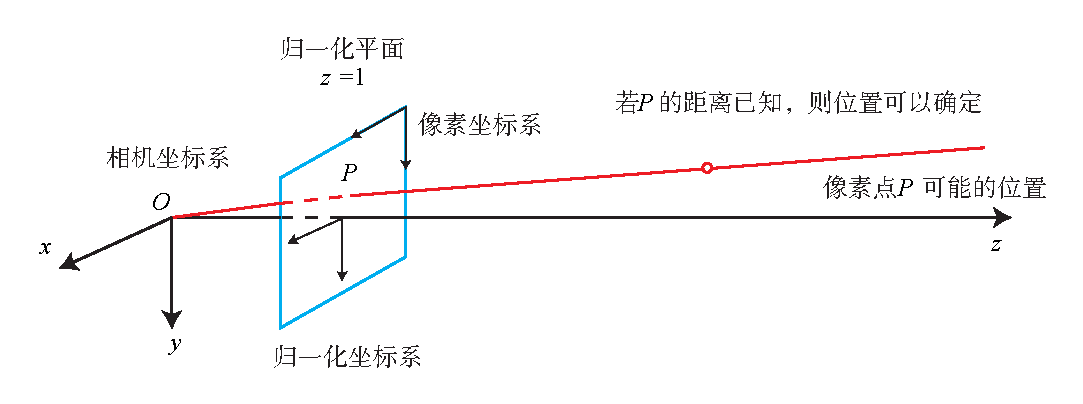
\includegraphics[width=1.0\textwidth]{chapter05/resources/cameraModel/pixelLocation.pdf}
	\caption{The location where the pixel may exist. }
	\label{fig:pixelLocation}
\end{figure}

There are many ways to measure the pixel distance (or depth). For example, the human eye can judge the distance of the object from us according to the difference of the scene (or parallax) seen by the left and right eyes. The principle of the binocular camera is also the same: the depth of each pixel is estimated by simultaneously acquiring the images of the left and right cameras and calculating the disparity between the images. The following is a brief introduction to the imaging principle of a binocular camera (such as \autoref{fig:stereoCamera}~).

A binocular camera generally consists of two horizontally placed cameras, a left eye camera and a right eye camera. Of course, you can also make up and down the two eyes \footnote{ then the appearance will be a bit strange. }, but the mainstream binoculars we have seen are all in the form of left and right. In the left and right binocular cameras, we can treat both cameras as pinhole cameras. They are placed horizontally, meaning that the center of the aperture of both cameras is on the $x$ axis. The distance between the two is called the \textbf{baseline} of the binocular camera (baseline, denoted as $b$), which is an important parameter of the binocular camera.

\begin{figure}[!ht]
	\centering
	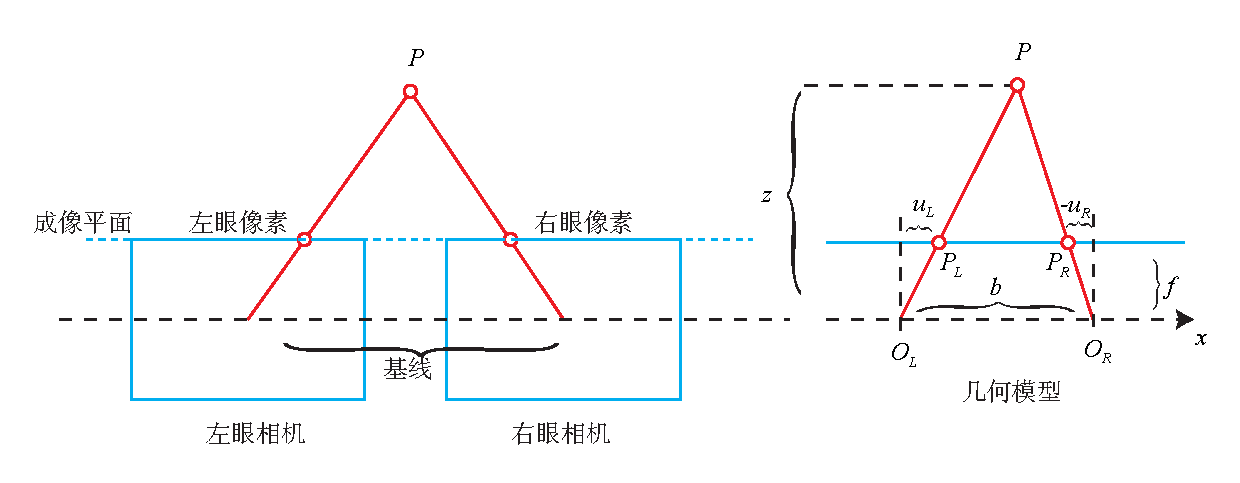
\includegraphics[width=1.0\textwidth]{chapter05/resources/cameraModel/stereoCamera.pdf}
	\caption{The imaging model of the binocular camera. $O_L, O_R$ is the center of the left and right apertures, the box is the imaging plane, and $f$ is the focal length. $u_L$ and $u_R$ are the coordinates of the imaging plane. Note that $u_R$ should be negative according to the coordinates defined in the figure, so the distance marked in the figure is $-u_R$. }
	\label{fig:stereoCamera}
\end{figure}

Now consider a space point $P$, which is a picture of the left eye camera and the right eye camera, denoted as $P_L, P_R$. These two imaging positions are different due to the presence of the camera baseline. Ideally, since the left and right cameras only have displacements on the $x$ axis, the image of $P$ differs only on the $x$ axis (corresponding to the $u$ axis of the image). Record its left coordinate is $u_L$, the right coordinate is $u_R$, and the geometric relationship is shown on the right side of \autoref{fig:stereoCamera}. According to the similar relationship between $\triangle PP_LP_R$ and $\triangle PO_LO_R$, there are:

\begin{equation}
\frac{{z - f}}{z} = \frac{{b - {u_L} + {u_R}}}{b}.
\end{equation}

Slightly sorted out, got:
\begin{equation}
z = \frac{{fb}}{d}, \quad d \buildrel \Delta \over = {u_L} - {u_R}.
\end{equation}

Where $d$ is defined as the difference between the abscissa of the left and right graphs, called \textbf{parparity}. Based on the parallax, we can estimate the distance between a pixel and the camera. Parallax is inversely proportional to distance: the larger the parallax, the closer the distance is to \footnote{the reader can simulate it with his own eyes. }. At the same time, since the parallax is at least one pixel, there is a theoretical maximum for the depth of the dual purpose, determined by $fb$. We see that the longer the baseline, the farther the maximum distance that binoculars can measure; conversely, small binoculars can only measure very close distances. Analogously, when we look at objects that are very far away (such as airplanes that are far away), we usually cannot accurately determine the distance.

Although the formula for calculating the depth from parallax is very simple, the calculation of the parallax $d$ itself is difficult. We need to know exactly where the pixel of the left eye image appears in the right eye image (ie, the correspondence), which is also a task that "humans find it easy and the computer finds it difficult". When we want to calculate the depth of each pixel, its calculation and precision will become a problem, and the parallax can only be calculated where the image texture changes. Due to the amount of computation, binocular depth estimation still requires real-time calculations using GPUs or FPGAs. This will be mentioned in Lecture 13.